\documentclass[../../main.tex]{subfiles}

\graphicspath{{../../image/}{../../figure/}}

\begin{document}

\section{有引导的扩散}\label{section:ch20-有引导的扩散}

到目前为止，我们讨论的扩散模型主要用于表示从一组训练样本 $\bm{x}_1,\cdots,\bm{x}_N$ 中学习到的无条件密度 $p(\bm{x})$，这些样本是独立地从 $p(\bm{x})$ 中抽取的。一旦模型训练好了，我们就可以从这个分布中生成新的样本。我们已经看到了一个从深度生成式模型中进行无条件采样的例子，用于人脸图像，如\cref{figure:ch01-生成人脸}所示，该例从一个 GAN 模型中进行采样。

然而在许多应用中，我们希望从条件分布 $p(\bm{x}\mid\bm{c})$ 中进行采样，其中条件变量 $\bm{c}$ 可以是一个类标签或是描述目标图像内容的文字。这也构成了诸如图像超分辨率、图像修复、视频生成等许多其他应用的基础。实现这一点的最简单方法是将 $\bm{c}$ 视为去噪神经网络 $\bm{g}(\bm{z},\bm{w},t,\bm{c})$ 的一个额外输入，然后使用匹配的 $\{\bm{x}_n,\bm{c}_n\}$ 对来训练网络。这种方法的主要问题是，网络可能会对条件变量赋予的权重不足，甚至忽略条件变量，因此我们需要一种方式来控制给予条件变量多少权重，并与样本多样性进行权衡。这种用以匹配条件信息的约束机制称为\textbf{引导}（guidance）。根据是否使用单独的分类器，引导主要有两种。

\begin{definition}[引导与引导尺度]\label{definition:ch20-引导}
设条件扩散模型的得分函数为 $\nabla_{\bm{x}}\ln p(\bm{x}\mid\bm{c})$。称在采样阶段人为放大条件项、以调节“条件信息权重”的机制为\textbf{引导}（guidance），其中用来控制条件项权重的超参数 $\lambda\geqslant0$ 称为\textbf{引导尺度}（guidance scale）。
\end{definition}

% SUPPLEMENT: parent=definition:ch20-引导; kind=motivation; location=紧随其后的 remark（重构新增）
\begin{remark}（重构新增）
引导要解决的问题是“条件不够强”：仅把 $\bm{c}$ 作为额外输入训练时，网络在训练集上可以完全忽略 $\bm{c}$ 而仍然取得不差的损失（因为无条件模型本身就是条件模型的一个特例），于是采样结果与 $\bm{c}$ 无关。引导通过在采样阶段人为放大条件项来补偿这一点，因此它改变的是\emph{采样}的分布，而不是训练的目标。\par
定义中的 $\lambda$ 是一个纯粹的采样超参数，不参与训练：同一组网络权重可以用不同的 $\lambda$ 生成不同“贴合度”的样本。这也意味着引导后的得分一般不再是某个归一化密度的得分（$\lambda\neq1$ 时它对应的是退火后的“尖锐化”分布），这一点在解释 $\lambda>1$ 的副作用时必须记住。\par
条件 $\lambda\geqslant0$ 只是约定；数学上 $\lambda<0$ 也有定义，但会主动\emph{远离}条件，实践中没有用处。下文会看到 $\lambda=0$ 与 $\lambda=1$ 是两个有明确概率含义的端点。
\end{remark}

\subsection{有分类器的引导}\label{subsection:ch20-有分类器的引导}

假设我们有一个训练好的分类器 $p(\bm{c}\mid\bm{x})$，下面从得分函数的角度考虑扩散模型。使用 Bayes 定理，我们可以将条件扩散模型的得分函数写成以下形式。

\begin{proposition}[分类器引导的得分分解]\label{proposition:ch20-分类器引导}
设 $p(\bm{x}\mid\bm{c})$、$p(\bm{x})$ 与 $p(\bm{c}\mid\bm{x})$ 为正的光滑密度，且 $p(\bm{c})$ 不依赖 $\bm{x}$。则
\begin{align}
\nabla_{\bm{x}}\ln p(\bm{x}\mid\bm{c})&=\nabla_{\bm{x}}\ln\Big\{\frac{p(\bm{c}\mid\bm{x})\,p(\bm{x})}{p(\bm{c})}\Big\}\nonumber\\
&=\nabla_{\bm{x}}\ln p(\bm{x})+\nabla_{\bm{x}}\ln p(\bm{c}\mid\bm{x}).
\label{align:ch20-条件得分}
\end{align}
\end{proposition}

\begin{proof}（重构新增）
由 Bayes 定理，$p(\bm{x}\mid\bm{c})=p(\bm{c}\mid\bm{x})p(\bm{x})/p(\bm{c})$。两边取对数得
\begin{align*}
\ln p(\bm{x}\mid\bm{c})=\ln p(\bm{c}\mid\bm{x})+\ln p(\bm{x})-\ln p(\bm{c}),
\end{align*}
再对 $\bm{x}$ 求梯度。由于 $p(\bm{c})$ 不依赖 $\bm{x}$，$\nabla_{\bm{x}}\ln p(\bm{c})=\bm{0}$，故\eqref{align:ch20-条件得分}成立。证毕。
\end{proof}

% SUPPLEMENT: parent=proposition:ch20-分类器引导; kind=motivation; location=紧随其后的 remark（重构新增）
\begin{remark}（重构新增）
\eqref{align:ch20-条件得分}把“条件生成”拆成“无条件生成 + 分类器梯度”两部分：第一项是常见的无条件得分函数，第二项推动去噪过程朝着最大化给定标签 $\bm{c}$ 在分类器模型下的概率的方向前进（Dhariwal and Nichol, 2021）。因此只要有任意一个训练好的无条件扩散模型和一个分类器，就能做条件采样，无需重新训练扩散模型——这是分类器引导最吸引人的地方。\par
$p(\bm{c})$ 不依赖 $\bm{x}$ 是推导的关键，也是“分类器只需给出似然比”的体现：分类器的绝对概率校准不影响引导方向，只有它对 $\bm{x}$ 的梯度起作用。$p(\bm{x}\mid\bm{c})$ 与 $p(\bm{c}\mid\bm{x})$ 都必须为正且可微，否则对数梯度无定义；在实践中这意味着分类器要在含噪样本上也有意义，而后文正是针对这一点提出批评。\par
\end{remark}

这里我们利用了 $\nabla_{\bm{x}}\ln p(\bm{c})=\bm{0}$，因为 $p(\bm{c})$ 不依赖于 $\bm{x}$。\eqref{align:ch20-条件得分}中的第一项是常见的无条件得分函数，第二项则推动去噪过程朝着最大化给定标签 $\bm{c}$ 在分类器模型下的概率的方向前进（Dhariwal and Nichol, 2021）。我们可以通过引入一个超参数 $\lambda$［称为引导尺度（guidance scale）］来控制赋予分类器梯度的权重。用于采样的得分函数随后变为
\begin{align}
\operatorname{score}(\bm{x},\bm{c},\lambda)=\nabla_{\bm{x}}\ln p(\bm{x})+\lambda\,\nabla_{\bm{x}}\ln p(\bm{c}\mid\bm{x}).
\label{align:ch20-分类器引导}
\end{align}
如果 $\lambda=0$，则恢复原始的无条件扩散模型；而如果 $\lambda=1$，则得到对应于条件分布 $p(\bm{x}\mid\bm{c})$ 的得分。当 $\lambda>1$ 时，模型被强烈引导遵守条件标签，我们也可能使用 $\lambda\geqslant1$ 的值，例如 $\lambda=10$。然而，这是以牺牲样本多样性为代价的，因为模型更倾向于“简单”的样本，即分类器能够正确分类的样本。

基于分类器的引导方法的一个问题是必须训练一个单独的分类器。此外，这个分类器需要能够对具有不同加噪程度的样本进行分类，而标准分类器是在干净的样本上进行训练的。因此，我们转向另一种无需独立分类器的引导方法，以避免使用单独的分类器。

\subsection{无分类器的引导}\label{subsection:ch20-无分类器的引导}

更进一步，我们无须分别训练多个网络来对 $p(\bm{x}\mid\bm{c})$ 和 $p(\bm{x})$ 进行建模，而是可以训练一个单独的条件模型，并在该模型中将条件变量 $\bm{c}$ 在训练过程中以一定概率设置为一个空值，例如 $\bm{c}=\bm{0}$，概率通常设置为 $10\%\sim20\%$。然后 $p(\bm{x})$ 由 $p(\bm{x}\mid\bm{c}=\bm{0})$ 表示。这在某种程度上类似于 dropout，dropout 会将一部分训练向量的所有条件输入都设为零（参见\cref{subsection:ch09-dropout}）。

训练完成后，得分函数\eqref{align:ch20-无分类器引导}用来强化条件信息的权重。实践表明，无分类器的引导相比有分类器的引导可以提供更高的生成质量（Nichol et al., 2021; Saharia et al., 2022）。原因是分类器 $p(\bm{c}\mid\bm{x})$ 可以忽略大部分输入向量 $\bm{x}$，只要能对 $\bm{c}$ 做出良好预测即可；而无分类器的引导基于条件密度 $p(\bm{x}\mid\bm{c})$，其必须为 $\bm{x}$ 的所有特征赋予高概率。

用\eqref{align:ch20-条件得分}替换\eqref{align:ch20-分类器引导}中的 $\nabla_{\bm{x}}\ln p(\bm{c}\mid\bm{x})$，即可得到如下结论（见\cref{exercise:ch20-20}）。

\begin{proposition}[无分类器引导（CFG）]\label{proposition:ch20-无分类器引导}
设条件得分与无条件得分分别为 $\nabla_{\bm{x}}\ln p(\bm{x}\mid\bm{c})$ 与 $\nabla_{\bm{x}}\ln p(\bm{x})$，且二者都存在。则对任意 $\lambda$，
\begin{align}
\operatorname{score}(\bm{x},\bm{c},\lambda)=\lambda\,\nabla_{\bm{x}}\ln p(\bm{x}\mid\bm{c})+(1-\lambda)\,\nabla_{\bm{x}}\ln p(\bm{x}).
\label{align:ch20-无分类器引导}
\end{align}
\end{proposition}

\begin{proof}（重构新增）
由\eqref{align:ch20-条件得分}得 $\nabla_{\bm{x}}\ln p(\bm{c}\mid\bm{x})=\nabla_{\bm{x}}\ln p(\bm{x}\mid\bm{c})-\nabla_{\bm{x}}\ln p(\bm{x})$。代入\eqref{align:ch20-分类器引导}：
\begin{align*}
\operatorname{score}&=\nabla_{\bm{x}}\ln p(\bm{x})+\lambda\big(\nabla_{\bm{x}}\ln p(\bm{x}\mid\bm{c})-\nabla_{\bm{x}}\ln p(\bm{x})\big)\\
&=\lambda\,\nabla_{\bm{x}}\ln p(\bm{x}\mid\bm{c})+(1-\lambda)\,\nabla_{\bm{x}}\ln p(\bm{x}),
\end{align*}
即\eqref{align:ch20-无分类器引导}。证毕。
\end{proof}

% SUPPLEMENT: parent=proposition:ch20-无分类器引导; kind=motivation; location=紧随其后的 remark（重构新增）
\begin{remark}（重构新增）
\eqref{align:ch20-无分类器引导}只用到条件模型自身的两个得分——条件得分与无条件得分——因此不需要任何外部分类器：训练时以一定概率把 $\bm{c}$ 置空，同一个网络就同时学会了二者。这是“无分类器”一词的确切含义。\par
对 $0<\lambda<1$，\eqref{align:ch20-无分类器引导}是条件对数密度 $\ln p(\bm{x}\mid\bm{c})$ 与无条件对数密度 $\ln p(\bm{x})$ 的凸组合，因而对应一个介于二者之间的“插值”分布；$\lambda=1$ 给出纯条件模型，$\lambda=0$ 给出纯无条件模型。对 $\lambda>1$，来自无条件得分项的系数 $1-\lambda$ 变为负值，模型主动降低那些忽略条件信息的样本的概率，而更倾向于生成考虑条件信息的样本。\par
注意 $\lambda\neq1$ 时\eqref{align:ch20-无分类器引导}一般不是某个归一化密度的得分（除非该插值恰好可积并归一化），所以“$\lambda>1$ 提高贴合度”是以偏离真实条件分布为代价的；这也解释了它为什么会让样本多样性下降。
\end{remark}

对于 $0<\lambda<1$，上式代表了条件对数密度 $\ln p(\bm{x}\mid\bm{c})$ 和无条件对数密度 $\ln p(\bm{x})$ 的凸组合；对于 $\lambda>1$，来自无条件得分项的贡献变为负值，这意味着模型主动降低了生成那些忽略条件信息的样本的概率，而更倾向于生成考虑条件信息的样本。

文本引导的扩散模型可以结合大语言模型的技术，把条件输入扩展为通用文本序列，即提示词（prompt），而非局限于预定义的类别标签（参见\cref{chapter:ch12-Transformer与注意力机制}）。这允许文本输入以两种方式影响去噪过程：第一，将基于 Transformer 的大语言模型的内部表示与去噪网络的输入连接起来；第二，允许去噪网络内的交叉注意力层关注文本标记序列。\cref{figure:ch20-文本引导}对基于文本提示的无分类器的引导做了说明。

\begin{figure}[htbp]
  \centering
  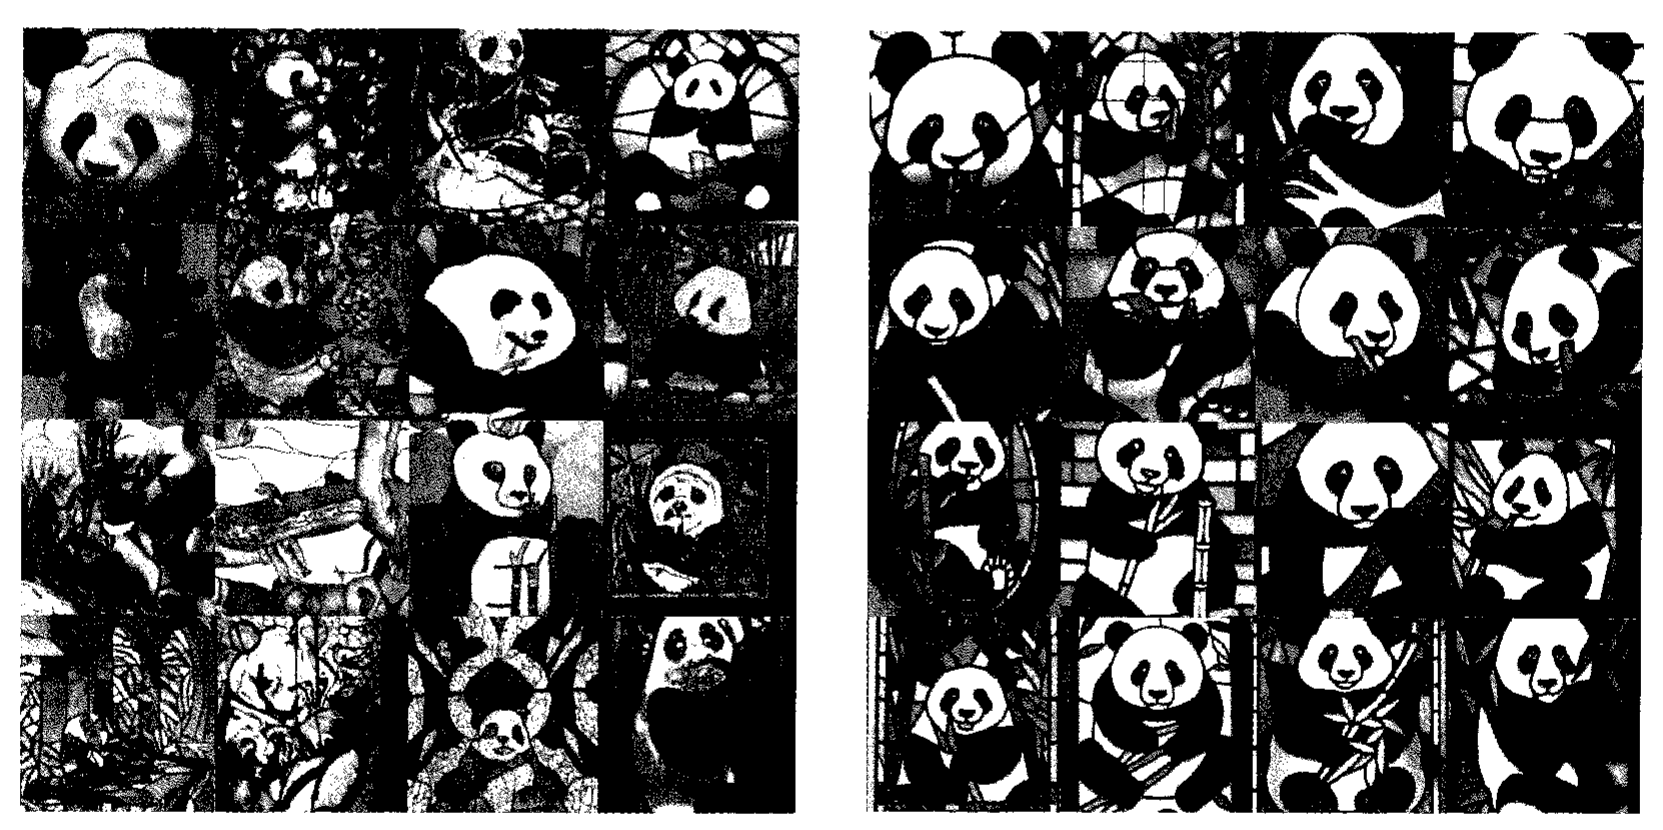
\includegraphics[width=0.9\textwidth]{ch20-fig20-7-cfg.png}
  \caption{基于文本提示的无分类器的引导，扩散模型由一个名为 GLIDE 的模型生成，使用的条件文本是“A stained glass window of a panda eating bamboo”（一只熊猫在吃竹子的彩绘玻璃窗）。左侧的样本是用 $\lambda=0$ 生成的（无引导，仅仅是纯条件模型），而右侧的样本是用 $\lambda=3$ 生成的［图片来源于 Nichol et al. (2021)，经授权使用］}
  \label{figure:ch20-文本引导}
\end{figure}

条件扩散模型的另一个应用是图像超分辨率，旨在将低分辨率图像转换为相应的高分辨率图像。这本质上是一个逆问题，单个低分辨率图像对应于多个高分辨率图像的解。实现方法是通过用低分辨率图像作为条件变量，对由 Gauss 分布采样生成的高分辨率样本进行去噪（Saharia, Ho, et al., 2021），参见\cref{figure:ch20-超分}。这些模型可以级联起来以实现非常高的图像分辨率（Ho et al., 2021），例如从 $64\times64$ 到 $256\times256$，然后从 $256\times256$ 到 $1024\times1024$。每个阶段通常用一个 U-Net 架构（参见\cref{subsection:ch10-U-Net架构}），且当前 U-Net 都以前一阶段的最终去噪结果为条件。

\begin{figure}[htbp]
  \centering
  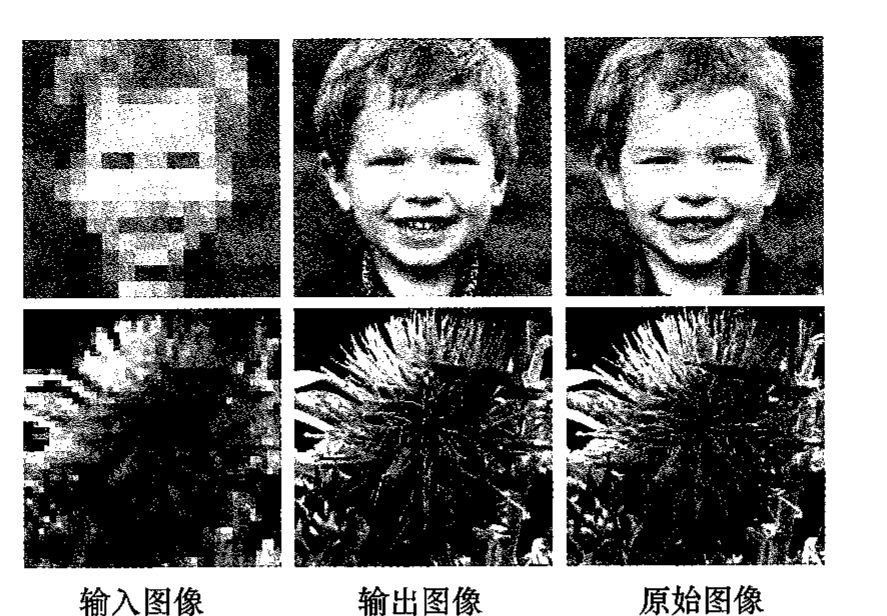
\includegraphics[width=0.68\textwidth]{ch20-fig20-8-superres.png}
  \caption{两个低分辨率图像以及由扩散模型生成的相应高分辨率图像。上面一行显示了一个 $16\times16$ 的输入图像和相应的 $128\times128$ 的输出图像，以及原始图像。下面一行显示了一个 $64\times64$ 的输入图像和一个 $256\times256$ 的输出图像，并与原始图像进行了对比［图片来源于 Saharia, Ho et al. (2021)，经授权使用］}
  \label{figure:ch20-超分}
\end{figure}

这种级联方式也适用于图像生成扩散模型，在这种模型中，首先在较低分辨率的图像上执行去噪操作，之后使用另一个独立的网络（可附加文本提示词输入）进行上采样，以生成最终的高分辨率图像（Nichol et al., 2021; Saharia et al., 2022）。由于去噪过程可能需要调用去噪网络数百次，与直接在高维空间中进行计算相比，级联方法能够大幅减少计算量。需要指出的是，这种方法依旧是在图像空间中直接进行操作的，只是分辨率较低而已。

对于在高分辨率图像空间中直接应用扩散模型所带来的高计算成本问题，另一种方法是使用\textbf{潜扩散模型}（latent diffusion model）（Rombach et al., 2021）。首先在无噪声图像上训练一个自编码器（autoencoder），以获得图像的低维表征并使参数固定操作。接下来训练一个 U-Net 网络，在低维空间中执行去噪操作，注意，这个空间本身并不能直接解释为图像。最后使用固定自编码器网络的输出部分将去噪表征映射到高分辨率图像空间。这种方法更有效地利用了低维空间，该空间可以专注于图像语义，并让解码器从去噪的低维表示中创建相应的清晰的高分辨率图像。

条件图像生成的其他应用还包括图像修复、去除裁剪、图像恢复、图像变形、图像风格转移、着色、去模糊和视频生成等（Yang, Srivastava, and Mandt, 2022）。\cref{figure:ch20-图像修复}展示了一个图像修复的例子。

\begin{figure}[htbp]
  \centering
  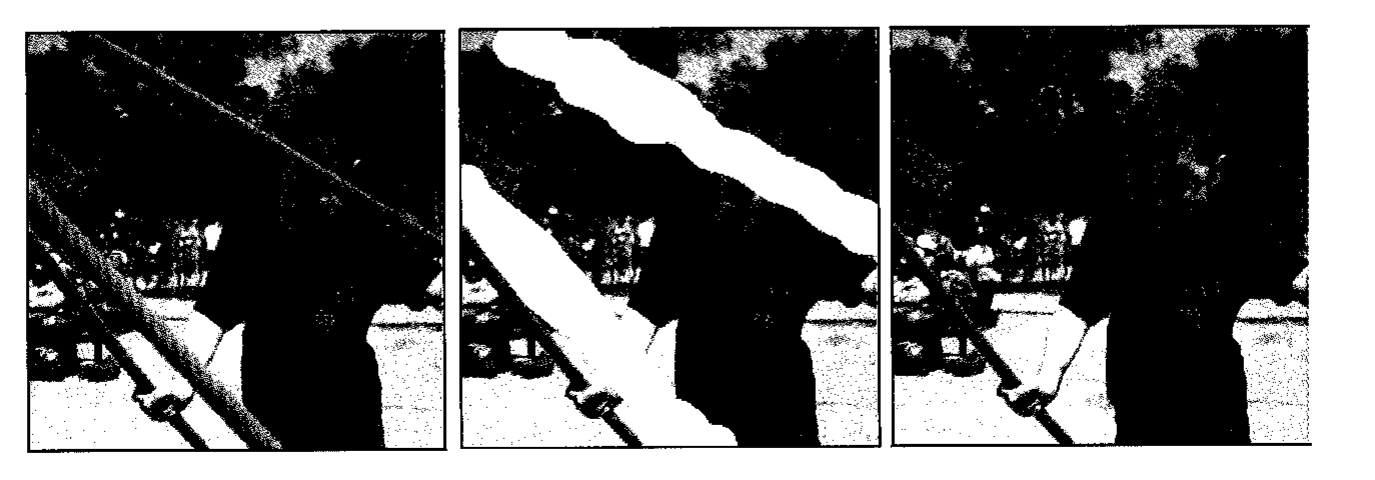
\includegraphics[width=0.9\textwidth]{ch20-fig20-9-inpainting.png}
  \caption{图像修复的一个例子。左侧是原始图像，中间是部分区域被移除的图像，右侧是经过修复处理的图像［图片来源于 Saharia, Chan, Chang et al. (2021)，经授权使用］}
  \label{figure:ch20-图像修复}
\end{figure}

\end{document}
